\documentclass{article}
\usepackage{amsmath,amsfonts,amsthm,amssymb}
\usepackage{setspace}
\usepackage{fancyhdr}
\usepackage{lastpage}
\usepackage{extramarks}
\usepackage{chngpage}
\usepackage{soul,color}
\usepackage{graphicx,float,wrapfig}
\usepackage{multirow, indentfirst}
\newcommand{\Class}{Introduction to Computer Science}
\newcommand{\ClassInstructor}{Longbo Huang}

% Homework Specific Information. Change it to your own
\newcommand{\Title}{Homework 1}
\newcommand{\DueDate}{Oct 7, 2013}         % Oct 11, 2006
\newcommand{\StudentName}{Luo Yuping}
\newcommand{\StudentClass}{JK30}
\newcommand{\StudentNumber}{2013011405}
\newcommand{\Grade}[ 1]{{\color{red} \bf {#1} points}}
\newcommand{\PS}[ 1]{{\color{red} \textbf{P.S.} \it {#1}}}

% In case you need to adjust margins:
\topmargin=-0.45in      %
\evensidemargin=0in     %
\oddsidemargin=0in      %
\textwidth=6.5in        %
\textheight=9.0in       %
\headsep=0.25in         %

% Setup the header and footer
\pagestyle{fancy}                                                       %
\lhead{\StudentName}                                                 %
\chead{\Title}  %
\rhead{\firstxmark}                                                     %
\lfoot{\lastxmark}                                                      %
\cfoot{}                                                                %
\rfoot{Page\ \thepage\ of\ \protect\pageref{LastPage}}                          %
\renewcommand\headrulewidth{0.4pt}                                      %
\renewcommand\footrulewidth{0.4pt}                                      %

%%%%%%%%%%%%%%%%%%%%%%%%%%%%%%%%%%%%%%%%%%%%%%%%%%%%%%%%%%%%%
% Some tools
\newcommand{\enterProblemHeader}[1]{\nobreak\extramarks{#1}{#1 continued on next page\ldots}\nobreak%
                                    \nobreak\extramarks{#1 (continued)}{#1 continued on next page\ldots}\nobreak}%
\newcommand{\exitProblemHeader}[1]{\nobreak\extramarks{#1 (continued)}{#1 continued on next page\ldots}\nobreak%
                                   \nobreak\extramarks{#1}{}\nobreak}%

\newcommand{\homeworkProblemName}{}%
\newcounter{homeworkProblemCounter}%
\newenvironment{homeworkProblem}[1][Problem \arabic{homeworkProblemCounter}]%
  {\stepcounter{homeworkProblemCounter}%
   \renewcommand{\homeworkProblemName}{#1}%
   \section*{\homeworkProblemName}%
   \enterProblemHeader{\homeworkProblemName}}%
  {\exitProblemHeader{\homeworkProblemName}}%

\newcommand{\homeworkSectionName}{}%
\newlength{\homeworkSectionLabelLength}{}%
\newenvironment{homeworkSection}[1]%
  {% We put this space here to make sure we're not connected to the above.

   \renewcommand{\homeworkSectionName}{#1}%
   \settowidth{\homeworkSectionLabelLength}{\homeworkSectionName}%
   \addtolength{\homeworkSectionLabelLength}{0.25in}%
   \changetext{}{-\homeworkSectionLabelLength}{}{}{}%
   \subsection*{\homeworkSectionName}%
   \enterProblemHeader{\homeworkProblemName\ [\homeworkSectionName]}}%
  {\enterProblemHeader{\homeworkProblemName}%

   % We put the blank space above in order to make sure this margin
   % change doesn't happen too soon.
   \changetext{}{+\homeworkSectionLabelLength}{}{}{}}%

\newcommand{\Answer}{\ \\\textbf{Answer:} }
\newcommand{\Acknowledgement}[1]{\ \\{\bf Acknowledgement:} #1}

%%%%%%%%%%%%%%%%%%%%%%%%%%%%%%%%%%%%%%%%%%%%%%%%%%%%%%%%%%%%%


%%%%%%%%%%%%%%%%%%%%%%%%%%%%%%%%%%%%%%%%%%%%%%%%%%%%%%%%%%%%%
% Make title
\title{\textmd{\bf \Class: \Title}\\{\large Instructed by \textit{\ClassInstructor}}\\\normalsize\vspace{0.1in}\small{Due\ on\ \DueDate}}
\date{}
\author{\textbf{\StudentName}\ \ \StudentClass\ \ \StudentNumber}
%%%%%%%%%%%%%%%%%%%%%%%%%%%%%%%%%%%%%%%%%%%%%%%%%%%%%%%%%%%%%

\begin{document}

\begin{spacing}{1.1}
\maketitle \thispagestyle{empty}

%%%%%%%%%%%%%%%%%%%%%%%%%%%%%%%%%%%%%%%%%%%%%%%%%%%%%%%%%%%%%
% Begin edit from here

Total: \Grade{96}

\begin{homeworkProblem}[Problem 3]
  \begin{itemize}
  \item[a.] If we were to purchase a flip-flop circuit from an electronic component store, we may find that it has an additional input called flip.  When this input changes from a 0 to 1, the output flips state (if it was 0 it is now 1 and vice versa). However, when the flip input changes from 1 to a 0, nothing happens.  Even though we may not know the details of the circuitry needed to accomplish this behavior, we could still use this device as an abstract tool in other circuits. Consider the circuitry using two of the following flip-flops.  If a pulse were sent on the circuit’s input, the bottom flip-flop would change state.  However, the second flip-flop would not change, since its input (received from the output of the NOT gate) went from a 1 to a 0.  As a result, this circuit would now produce the outputs 0 and 1. A second pulse would flip the state of both flip-flops, producing an output of 1 and 0. What would be the output after a third pulse? After a fourth pulse?

   \begin{center}
     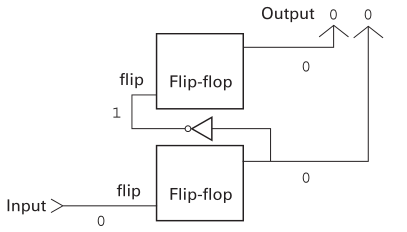
\includegraphics[scale = 0.5]{images/P3-a.png}
   \end{center}

  \item[b.] It is often necessary to coordinate activities of various components within a computer.  This is accomplished by connecting a pulsating signal (called a clock) to circuitry similar to part a. Additional gates (as shown) will then send signals in a coordinated fashion to other connected circuits.  On studying this circuit you should be able to confirm that on the $1^{st} , 5^{th} , 9^{th}$ ... pulses of the clock, a 1 will be sent on output A.  On what pulses of the clock will a 1 be sent on output B? On what pulses of the clock will a 1 be sent on output C? On which output is a 1 sent on the 4 th pulse of the clock?
   
    \begin{center}
      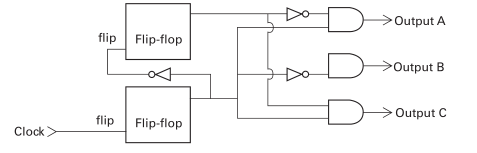
\includegraphics[scale = 0.5]{images/P3-b.png}
    \end{center}
  \end{itemize}

  \Answer 
  \begin{itemize}
  \item[a.] After a third pulse, the output will be 1 and 1. After a fourth pulse, the output will be 0 and 0. \Grade{4}

  \item[b.] On the $2^{nd}, \,4^{th}, \,6^{th}, \dots$ pulses of the clock, a 1 will be sent on output B. On the $3^{rd}, \, 7^{th}, \, 11^{th}, \dots$ pulses of the clock, a 1 will be sent on output C. On the $4^{th}$ pulse of the clock a 1 is sent on output B.  \Grade{5}

  \end{itemize}
\end{homeworkProblem}

\begin{homeworkProblem}[Problem 6]
  How many cells can be in a computer’s main memory if each cell’s address can be repre- sented by two hexadecimal digits? What if four hexadecimal digits are used?

  \Answer If each cell's address can be represented by 2 hexadecimal digits, 256 cells can be in a computer's main memory. For 4 hexadecimal digits used, the answer is 65536. \Grade{9}
\end{homeworkProblem}

\begin{homeworkProblem}[Problem 9]
  Express the following bit patterns in hexadecimal notation:

  \begin{itemize}
  \item [a.] \texttt{101000001010}
  \item [b.] \texttt{110001111011}
  \item [c.] \texttt{000010111110}
  \end{itemize}

  \Answer 
  \begin{itemize}
  \item[a.] $\texttt{(101000001010)}_2 = \texttt{0xA0A}$ \Grade{3}
  \item[b.] $\texttt{(110001111011)}_2 = \texttt{0xC7B}$ \Grade{3}
  \item[c.] $\texttt{(000010111110)}_2 = \texttt{0xBE}$ \Grade{2}
  \end{itemize}

\end{homeworkProblem}


\begin{homeworkProblem}[Problem 15]
  How many bytes of storage space would be required to store a 400-page novel in which each page contains 3500 characters if ASCII were used? How many bytes would be required if Unicode were used?
  
  \Answer 1400000 bytes will be needed for ASCII. 2800000 bytes will be needed for Unicode. \Grade{4+5=9}
  
\end{homeworkProblem}


\begin{homeworkProblem}[Problem 19]
  Here is a message in ASCII. What does it say?

  \texttt{01010111 01101000 01100001 01110100 00100000 01100100 01101111 01100101 01110011 00100000 01101001 01110100 00100000 01110011 01100001 01111001 00111111}
  
  \Answer ``What does it say?'' \Grade{9}
  
\end{homeworkProblem}


\begin{homeworkProblem}[Problem 26]
  Convert each of the following binary representations to its equivalent base ten representation:

  \texttt{a. 1111 b. 0001 c. 10101 d. 1000 e. 10011 f. 000000 g. 1001 h. 10001 i. 100001 j. 11001 k. 11010 l. 11011}
  
  \Answer 
  \Grade{10}
  \begin{itemize}
  \item[a:] 15
  \item[b:] 1
  \item[c:] 21
  \item[d:] 8
  \item[e:] 19
  \item[f:] 0
  \item[g:] 9
  \item[h:] 17
  \item[i:] 33
  \item[j:] 25
  \item[k:] 26
  \item[l:] 27
  \end{itemize}
  
\end{homeworkProblem}


\begin{homeworkProblem}[Problem 33]
  Solve each of the following problems by translating the values into two’s complement notation (using patterns of 5 bits), converting any subtraction problem to an equivalent addition problem, and performing that addition. Check your work by converting your answer to base ten notation. (Watch out for overflow.)

  \begin{center}
    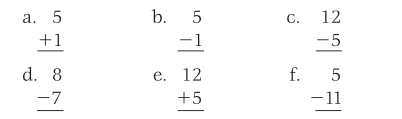
\includegraphics[scale = 0.7]{images/P33.png}
  \end{center}
  
  \Answer 

  \Grade{6} \PS{-3 for no decimal represention. I don't know how many points this should deduct. I've sent emails to both of TAs but neither of them replied.}

  {\tt
    \begin{tabular}{l @{} r l @{} r l @{} r}
      a. &  00101 & b. &  00101 & c. &  01100 \\
         & +00001 &    & +11111 &    & +11011 \\ \cline{2-2} \cline{4-4} \cline{6-6}
         &  00110 &    &  00100 &    &  00111 \\
      d. &  01000 & e. &  01100 & f. &  00101 \\
         & +11001 &    & +00101 &    & +10101 \\ \cline{2-2} \cline{4-4} \cline{6-6}
         &  00001 &    &  10001 &    &  11010 
    \end{tabular}
  }
  
\end{homeworkProblem}


\begin{homeworkProblem}[Problem 42]
  One of the bit patterns 01011 and 11011 represents a value stored in excess 16 notation and the other represents the same value stored in two’s complement notation.

a. What can be determined about this common value?

b. What is the relationship between a pattern representing a value stored in two’s complement notation and the pattern representing the same value stored in excess notation when both systems use the same bit pattern length?
  
  \Answer 
  a. It must be 11 or -5. \Grade{4}
  
  b. They are different in high-order end and are the same at the other positions. \Grade{5}
  
\end{homeworkProblem}


\begin{homeworkProblem}[Problem 47]
  What would be the encoded version of the message

  \texttt{xxy yyx xxy xxy yyx}

  if LZW compression, starting with the dictionary containing x, y, and a space (as described in Section 1.8), were used?
  
  \Answer \texttt{1123221343435} \Grade{9}
  
\end{homeworkProblem}

\begin{homeworkProblem}[Problem 52]
  The following message was originally transmitted with odd parity in each short bit string. In which strings have errors definitely occurred?

  \texttt{11001 11011 10110 00000 11111 10001 10101 00100 01110}
  
  \Answer In \texttt{11011, 00000, 10001}. \Grade{9}
  
\end{homeworkProblem}


\begin{homeworkProblem}[Problem 54]
  Using the error-correcting code described in Figure 1.30, decode the following words:
  
  \Answer 
  \begin{itemize}
  \item[a.] \texttt{HE} \Grade{1}
  \item[b.] \texttt{FED} \Grade{1}
  \item[c.] \texttt{DEAD} \Grade{2}
  \item[d.] \texttt{CABBAGE} \Grade{3}
  \item[e.] \texttt{CAFE} \Grade{2}
  \end{itemize}
  
\end{homeworkProblem}


% \Acknowledgement{Thank XXX XX 2004010102 and XXX XXXX 2004010103 for the discussion about ...}

% End edit to here
%%%%%%%%%%%%%%%%%%%%%%%%%%%%%%%%%%%%%%%%%%%%%%%%%%%%%%%%%%%%%

\end{spacing}
\end{document}

%%%%%%%%%%%%%%%%%%%%%%%%%%%%%%%%%%%%%%%%%%%%%%%%%%%%%%%%%%%%%
